\documentclass[twocolumn,
			   showpacs,%
               nofootinbib,
               aps,%
               %eqsecnum,
               prd,
               notitlepage,
               showkeys,
               10pt]{revtex4-1}
               
%Loading my personal settings
\usepackage{todonotes}

%math and formulas
\usepackage{amssymb}
\usepackage{amsmath}
\usepackage{physics}

%language settings and microtype
\usepackage[english]{babel}
\usepackage{microtype}

%useful packages
\usepackage{graphicx}
\usepackage{siunitx}
\usepackage{xcolor}
\usepackage{float}
\usepackage{dcolumn}
\usepackage{blindtext}
\usepackage{xfrac}
\usepackage[labelfont=bf]{caption}
\usepackage{subcaption}


%feynman diagrams
\usepackage{tikz}
\usepackage{tikz-feynman}
\tikzfeynmanset{compat=1.0.0} 

%loading the `external` library
\usetikzlibrary{external}   
%Create directory to store the diagrams and all related files          
\immediate\write18{mkdir -p feynman-diagrams} 
% Activate externalization
\tikzexternalize[
  %Avoid cluttering the directory                     
  prefix=feynman-diagrams/, 
  %Calling lualatex externally
  system call={             
    lualatex \tikzexternalcheckshellescape -halt-on-error -interaction=batchmode -jobname="\image" "\texsource"  || rm "\image.pdf"
  },
]

%color settings
\definecolor{mydarkblue}{RGB}{1,1,141}

%correcting parindent
\setlength{\parindent}{0pt}


%always use hyperref at the end of the preamble!
\usepackage[colorlinks=True]{hyperref}
\hypersetup{allcolors=mydarkblue}

%main document
\begin{document}

%Personel data
\title{F91: Studying the $Z$ boson with the ATLAS Detector at the LHC }
\author{Mathieu Kaltschmidt}
\email{M.Kaltschmidt@stud.uni-heidelberg.de}
\affiliation{Heidelberg University,  D-69117 Heidelberg, Germany}
\author{Quirinus Schwarzenb\"ock}
\email{Schwarzenb\"ock@stud.uni-heidelberg.de}
\affiliation{Heidelberg University,  D-69117 Heidelberg, Germany}

\date[Carried out in the week of  ]{March 4$^{\text{th}}$, 2019}


\begin{abstract}
This experiment has been performed as part of the advanced lab course for physics students (FP) at Heidelberg University.
The goal of this computer-based experiment was to determine the invariant mass spectrum for the $Z$ boson using data acquired by the Large Hadron Collider at CERN in Geneva.
\end{abstract}

\maketitle



\section{Introduction}
Taking the geometric properties into account, it is very easy to see the following connection between momentum and transversal momentum
\begin{align}
	p_x &= p_T \cos(\phi)\\
	p_y &= p_T \sin(\phi)\\
	p_z \tan(\theta) &= p_T
\end{align}
From the definition of the pseudorapidity (eq: \ref{pseudorapidity}) we have $\theta = 2\arctan(e^{-\eta})$. Using the identity $\tan(2\arctan(x)) = \frac{2x}{1 - x^2}$, these equations lead to 
\begin{align}
	p_z &= p_T\sinh(\eta)\\
	\left|\mathbf{p}\right| &= p_T \cosh(\eta)
\end{align}



Already implementing the formulas mentioned in the theory part of \cite{F91manual} to speed things up a little.
\begin{align}
\mathcal{L} = \frac{N_1N_2f_{\text{rev}}n_b}{4\pi\sigma_x\sigma_y}
\end{align}

\blindtext

\begin{align}
\mathcal{L}_{\text{int}} = \int \mathcal{L} \ \dd t	
\end{align}

\blindtext

\begin{align}
N = \sigma_{pp\rightarrow X} \cdot \mathcal{L}_{\text{int}}
\end{align}


\section{Theory}


\begin{figure}[H]
\centering	
\feynmandiagram [small] [horizontal' = a to b] {
	i1 [particle=\(\overline{u}\)] -- [fermion] a  -- [fermion] i2 [particle=\(d\)],
	a -- [photon, edge label=\(W^{-}\)] b ,
	f1 [particle=\(\nu_{e^{-}}\)] -- [fermion] b -- [fermion] f2 [particle=\(e^{-}\)],
	};
\caption{1-Lepton final state.}
\end{figure}

\begin{figure}[H]
\centering	
\feynmandiagram [small] [horizontal' = a to b] {
	i1 [particle=\(q\)] -- [fermion] a  -- [fermion] i2 [particle=\(\overline{q}\)],
	a -- [photon, edge label=\(\gamma / Z^0\)] b ,
	f1 [particle=\(e^{+}\)] -- [fermion] b -- [fermion] f2 [particle=\(e^{-}\)],
	};
\caption{2-Lepton final state.}
\end{figure}

\begin{figure}[H]
\centering	
\begin{tikzpicture}
\feynmandiagram{
    \vertex (a) {\(d\)};
    \vertex [right=of a] (b);
    \vertex [above right=of b] (c);
    \vertex [above right=of c] (f1) {\(e^{-}\)};
    \vertex [below right=of c] (f2) {\(\overline{\nu}_{e^{-}}\)};
    \vertex [below =of a] (d) {\(\overline{u}\)};
    \vertex [right=of d] (e);
    \vertex [below right=of e] (f);
     \vertex [above right=of f] (f3) {\(e^{-}\)};
    \vertex [below right=of f] (f4) {\(e^{+}\)};

 
    \diagram* {
      (a) -- [fermion] (b) -- [boson, edge label=\(W^{-}\)] (c),
      (d) -- [anti fermion] (e) -- [boson, edge label'=\(Z^{0}\)] (f),
      (f1) -- [anti fermion] (c) -- [anti fermion] (f2),
      (f3) -- [anti fermion] (f) -- [anti fermion] (f4),
      
      (b) -- [edge label' = \(\overline{u}\) ] (e),
};
}
\end{tikzpicture}
\caption{3-Lepton final state.}
\end{figure}


\section{Experiment}

\begin{figure}[H]
\centering
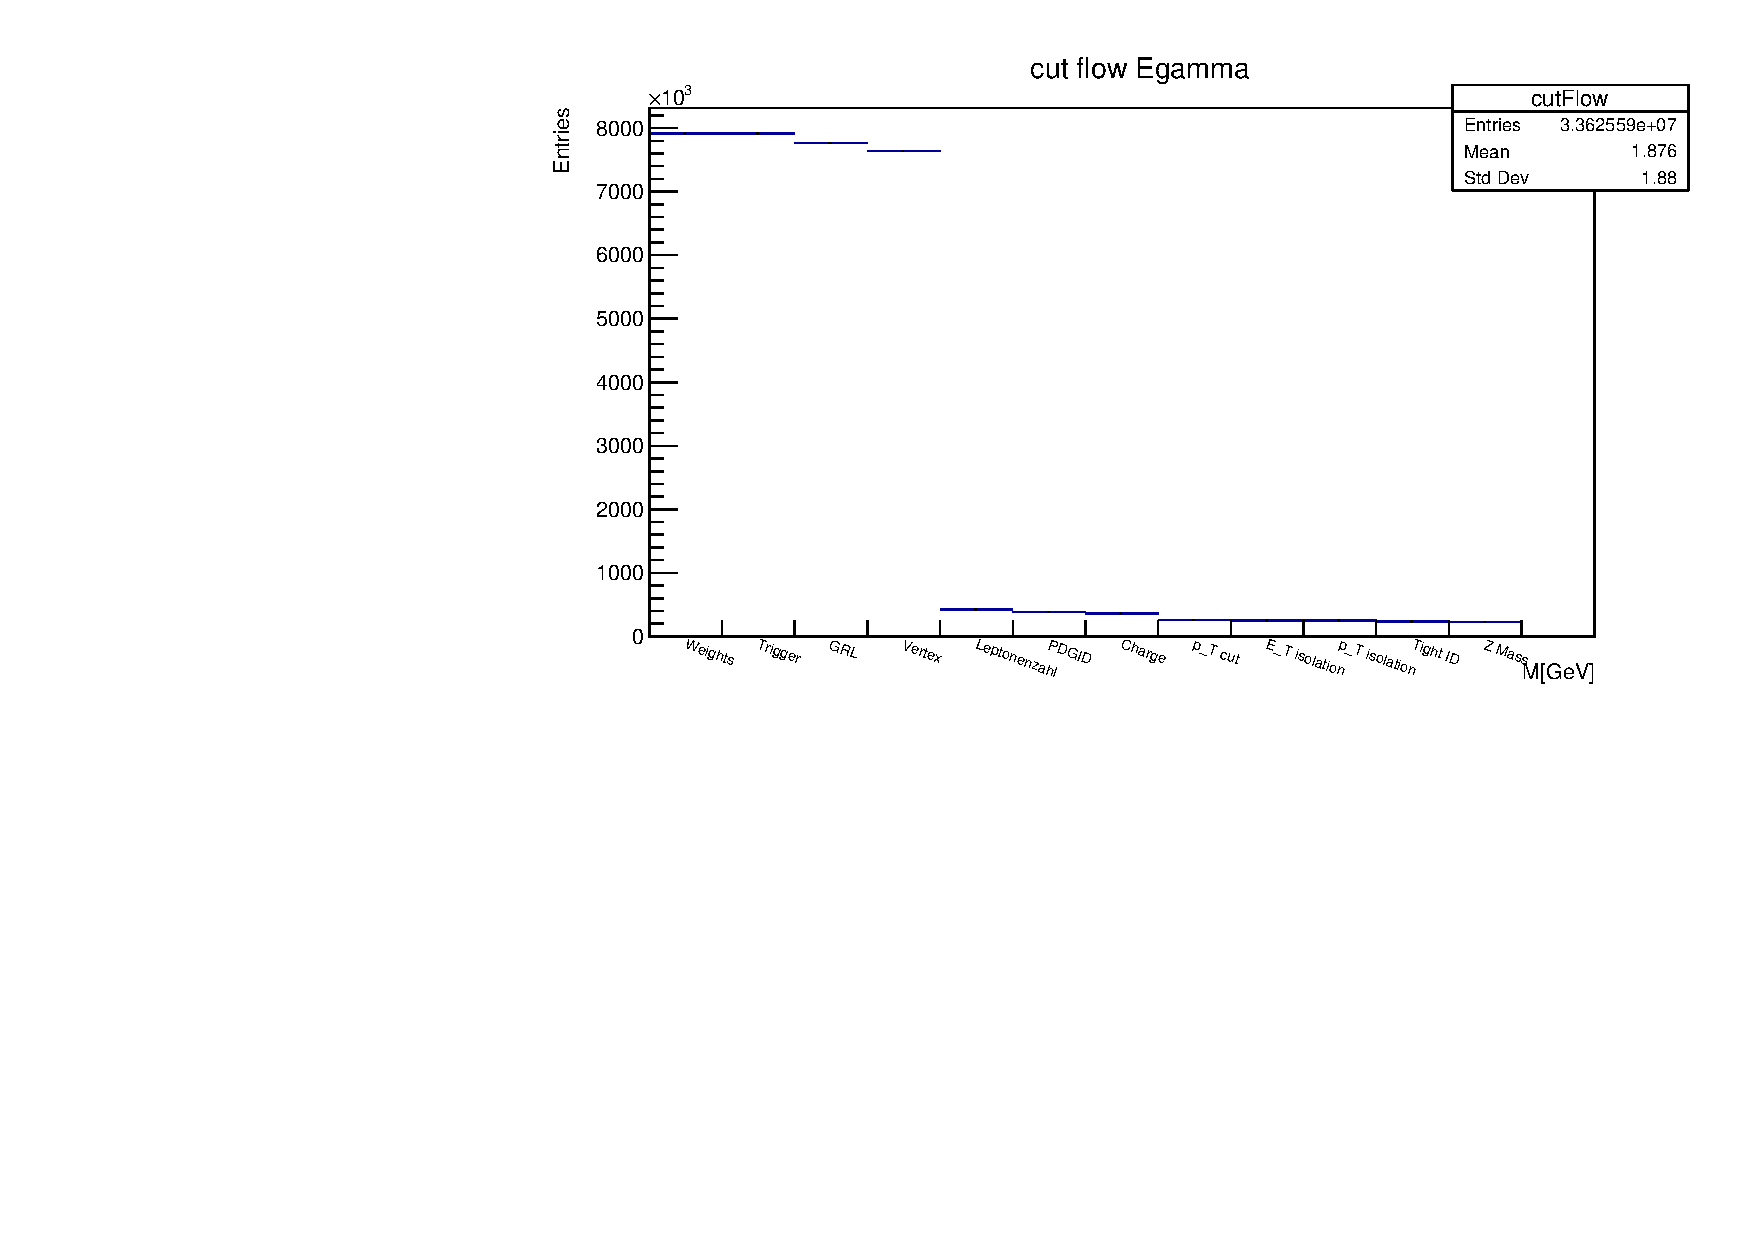
\includegraphics[width = 0.45\textwidth]
{figures/plots/CutFlow}
\caption{Cut flow diagram for our event selection algorithm.}	
\end{figure}




\blindtext




\section{Results}
\blindtext



\begin{figure}[H]
	\centering
	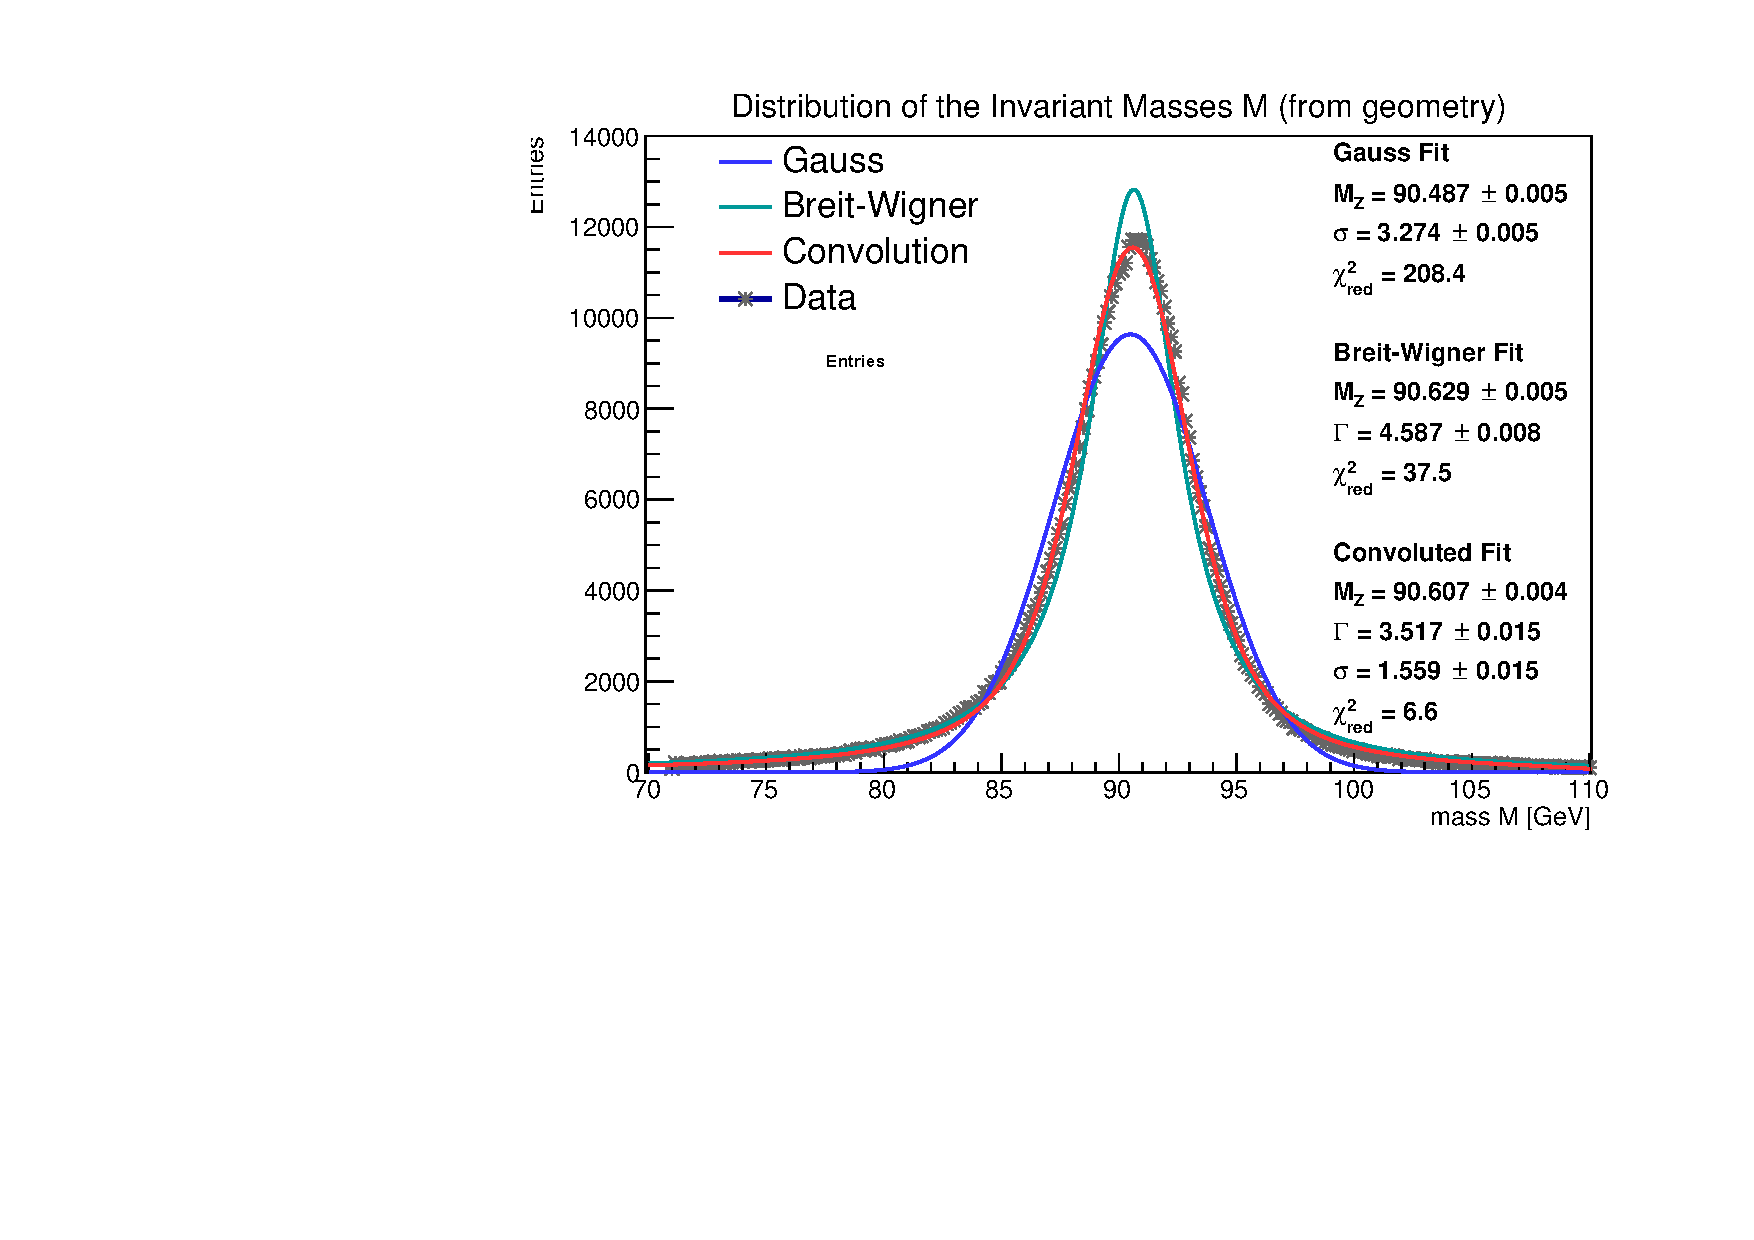
\includegraphics[width = 0.45\textwidth]{figures/plots/ZMassFitted}
	\caption{Distribution of the $Z$ masses $M_z$ with Gau\ss, Breit-Wigner and a convoluted fit.}
\end{figure}




\section{Discussion}

\Blindtext


\begin{acknowledgments}

We would like to thank our supervisor Philipp Ott for his guidance throughout the operation of this experiment.

\end{acknowledgments}

\bibliographystyle{abbrv}
\bibliography{bibliography/literatur}
\nocite{*}

\end{document}
